\documentclass[a4paper,12pt]{article}

\author{\textbf{Софиа Белен Лопес Висенс}\\
Группа Б02-903\\
\large Московский физико-технический институт}
\title{\textbf{Задание 1}\\
Параллельное умножение матриц}
\date{}

\usepackage[margin=0.9in]{geometry}
\usepackage{graphicx}
\usepackage{float}
\usepackage[utf8]{inputenc}
\usepackage[T2A]{fontenc}
\usepackage{textcomp}
\usepackage{amsmath, amssymb}
\usepackage{siunitx}
\usepackage{subcaption}
\usepackage{multirow}

\renewcommand{\figurename}{Рис.}
\renewcommand{\tablename}{Таблица}
\renewcommand*\contentsname{Содержание}

\begin{document}
\maketitle
\newpage

\section{Параллельное умножение матриц DGEMM}

\begin{verbatim}
#pragma omp parallel for collapse(3) num_threads(P)
for (int j = 0; j < n; j++)
    for (int i = 0; i < l; i++)
        for (int k = 0; k < m; k++)
            C[i + j * l] += A[i + k * l] * B[k + j * m];
\end{verbatim}

\section{Анализ сильной/слабой масштабируемости}

\begin{itemize}
    \item Сильная масштабируемость — показывает, как меняется время решения задачи с увеличением количества процессоров (или вычислительных узлов) при неизменном общем объёме задачи.

\item Слабая масштабируемость — показывает, как меняется время решения задачи с увеличением количества процессоров (узлов) при неизменном объёме задачи для одного процессора (или узла).
\end{itemize}

Из графики видно 

\begin{figure}[H]
    \centering
    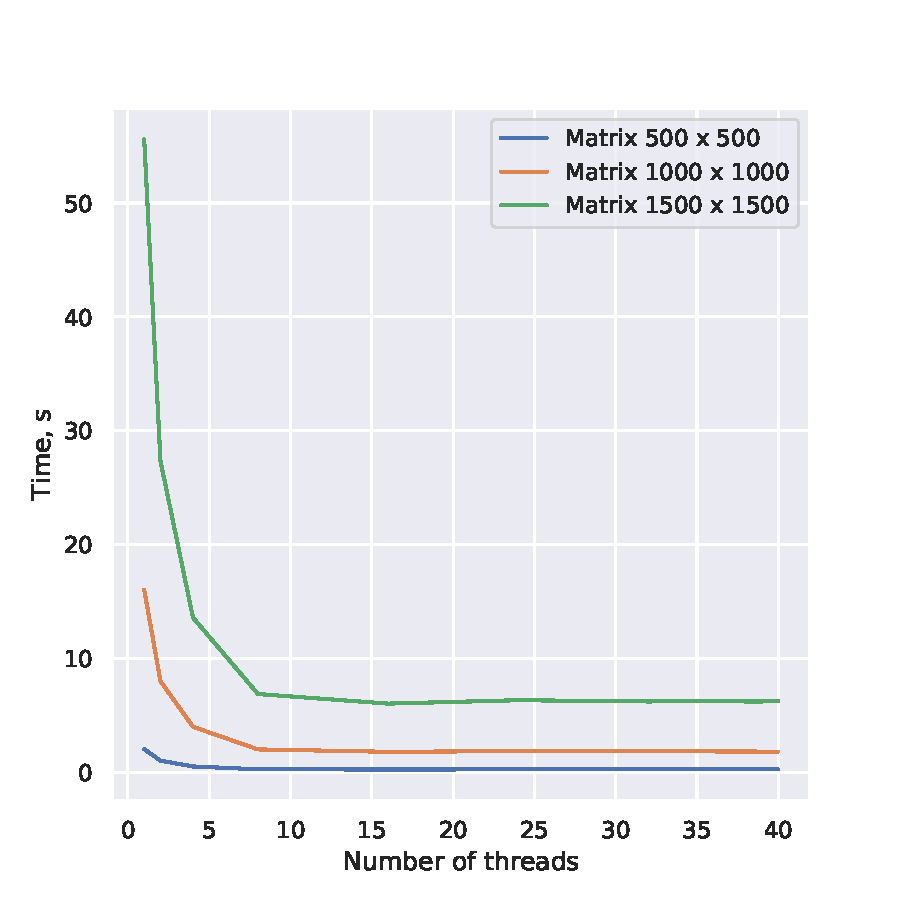
\includegraphics[width=0.8\textwidth]{../img/graph1.pdf}
    % \caption{../img/graph1.pdf}
    \label{fig:-img-graph1-pdf}
\end{figure}

\section{Оптимизации под узлы суперкомпьютера МФТИ}

\end{document}

